%%%%%%%%%%%%%%%%%%%%%%%%%%%%%%%%%%%%%%%%%
% Weekly Report 
% LaTeX Template
% Version 1.3 (19/10/24)
% Modified by
% Enes TAŞTAN
% Erdem TUNA
% Halil TEMURTAŞ
%%%%%%%%%%%%%%%%%%%%%%%%%%%%%%%%%%%%%%%%%
%
%----------------------------------------------------------------------------------------
%	PACKAGES AND OTHER DOCUMENT CONFIGURATIONS
%----------------------------------------------------------------------------------------
\documentclass[a4paper,12pt]{article}
%-----packages------
\usepackage[a4paper, total={6.2in, 8.5in}, headheight=110pt]{geometry}
\usepackage[english]{babel}
\usepackage[utf8x]{inputenc}
\usepackage{amsmath}
\usepackage{graphicx}
\usepackage[colorinlistoftodos]{todonotes}
\usepackage{gensymb} % this could be problem
\usepackage{float}
\usepackage{fancyref}
\usepackage{subcaption}
\usepackage[toc,page]{appendix} %appendix package
\usepackage{xcolor}
\usepackage{listings}


\usepackage[export]{adjustbox}

\usepackage{xspace}
\usepackage{amssymb}
\usepackage{nicefrac}
\usepackage{gensymb}
\usepackage{fancyhdr}
\usepackage{lipsum}  % for lipsum
\usepackage[final]{pdfpages}  % pdf include
\usepackage{array} %allows more options in tables
\usepackage{pgfplots,pgf,tikz} %coding plots in latex
\usepackage{capt-of} % allows caption outside the figure environment
\usepackage[export]{adjustbox} %more options for adjusting the images
\usepackage{multicol,multirow,slashbox} % allows tables like table1
%\usepackage[hyperfootnotes=false]{hyperref} % clickable references
\usepackage{epstopdf} % useful when matlab is involved
%\usepackage{placeins} % prevents the text after figure to go above figure with \FloatBarrier 
%\usepackage{listingsutf8,mcode} %import .m or any other code file mcode is for matlab highlighting

%-----end of packages

%-----specifications-----
\definecolor{mGreen}{rgb}{0,0.6,0} % for python
\definecolor{mGray}{rgb}{0.5,0.5,0.5}
\definecolor{mPurple}{rgb}{0.58,0,0.82}
\definecolor{mygreen}{RGB}{28,172,0} % color values Red, Green, Blue for matlab
\definecolor{mylilas}{RGB}{170,55,241}

\setcounter{secnumdepth}{5} % how many sectioning levels to assign numbers to
\setcounter{tocdepth}{5}    % how many sectioning levels to show in ToC

\lstdefinestyle{CStyle}{
	commentstyle=\color{mGreen},
	keywordstyle=\color{magenta},
	numberstyle=\tiny\color{mGray},
	stringstyle=\color{mPurple},
	basicstyle=\footnotesize,
	breakatwhitespace=false,         
	breaklines=true,
	frame=single,
	rulecolor=\color{black!40},                 
	captionpos=b,                    
	keepspaces=true,                 
	numbers=left,                    
	numbersep=5pt,                  
	showspaces=false,                
	showstringspaces=false,
	showtabs=false,                  
	tabsize=2,
	language=C
}

\lstset{language=Matlab,%
	%basicstyle=\color{red},
	breaklines=true,%
	frame=single,
	rulecolor=\color{black!40},
	morekeywords={matlab2tikz},
	keywordstyle=\color{blue},%
	morekeywords=[2]{1}, keywordstyle=[2]{\color{black}},
	identifierstyle=\color{black},%
	stringstyle=\color{mylilas},
	commentstyle=\color{mygreen},%
	showstringspaces=false,%without this there will be a symbol in the places where there is a space
	numbers=left,%
	numberstyle={\tiny \color{black}},% size of the numbers
	numbersep=9pt, % this defines how far the numbers are from the text
	emph=[1]{for,end,break},emphstyle=[1]\color{red}, %some words to emphasise
	%emph=[2]{word1,word2}, emphstyle=[2]{style},    
}


\tikzset{
	desicion/.style={
		diamond,
		draw,
		text width=4em,
		text badly centered,
		inner sep=0pt
	},
	block/.style={
		rectangle,
		draw,
		text width=10em,
		text centered,
		rounded corners
	},
	cloud/.style={
		draw,
		ellipse,
		minimum height=2em
	},
	descr/.style={
		fill=white,
		inner sep=2.5pt
	},
	connector/.style={
		-latex,
		font=\scriptsize
	},
	rectangle connector/.style={
		connector,
		to path={(\tikztostart) -- ++(#1,0pt) \tikztonodes |- (\tikztotarget) },
		pos=0.5
	},
	rectangle connector/.default=-2cm,
	straight connector/.style={
		connector,
		to path=--(\tikztotarget) \tikztonodes
	}
}

\tikzset{
	desicion/.style={
		diamond,
		draw,
		text width=4em,
		text badly centered,
		inner sep=0pt
	},
	block/.style={
		rectangle,
		draw,
		text width=10em,
		text centered,
		rounded corners
	},
	cloud/.style={
		draw,
		ellipse,
		minimum height=2em
	},
	descr/.style={
		fill=white,
		inner sep=2.5pt
	},
	connector/.style={
		-latex,
		font=\scriptsize
	},
	rectangle connector/.style={
		connector,
		to path={(\tikztostart) -- ++(#1,0pt) \tikztonodes |- (\tikztotarget) },
		pos=0.5
	},
	rectangle connector/.default=-2cm,
	straight connector/.style={
		connector,
		to path=--(\tikztotarget) \tikztonodes
	}
}
%-----end of specifications-----


%----commands----
\newcommand\nd{\textsuperscript{nd}\xspace}
\newcommand\rd{\textsuperscript{rd}\xspace}
\newcommand\nth{\textsuperscript{th}\xspace} %\th is taken already
\newcommand{\specialcell}[2][c]{ \begin{tabular}[#1]{@{}c@{}}#2\end{tabular}} % for too long table lines

\newcommand{\blankpage}{
	\- \\[9cm]	
	{ \centering \textit{This page intentionally left blank.} \par }
	\- \\[9cm]
}% For Blank Page

\makeatletter
\renewcommand\paragraph{\@startsection{paragraph}{4}{\z@}%
	{-2.5ex\@plus -1ex \@minus -.25ex}%
	{1.25ex \@plus .25ex}%
	{\normalfont\normalsize\bfseries}}
\makeatother
%-----end of commands-----


\pagestyle{fancy}
\setlength\headheight{150pt}
\setlength{\footskip}{2.5cm}
%\fancyhead[LO,LE]{Duayenler Ltd. Şti.}
%\fancyhead[RO,RE]{October 19, 2018}
\fancyhead[LO,LE]{\textbf{Project:} IOT Distributed Temperature\\ Measurement and Control (Control Lab) }
\fancyhead[RO,RE]{Erdem Tuna\\2167419}

%\fancyhead[RO]{Sarper Sertel (05435156039),\\Enes Taştan (05436834336), Erdem Tuna (05352563320),\\Halil Temurtaş (05316322194), İlker Sağlık (05417229573)}
%\rfoot{\includegraphics[width=2.2cm]{../../../Documents/logos/logo2-page-with-stroke}}

\begin{document}
	



%\begin{figure}[ht]
%	\begin{minipage}[]{0.65\textwidth}
%		\begin{flushleft}
%			%\vspace*{-.7cm}
%\Large\textbf{A Search on Transducers for Ambient Noise Measurements}
%	\end{flushleft}		
%\end{minipage}
%\begin{minipage}[]{0.35\textwidth}
%	\begin{flushright}
%		\includegraphics[width=5cm,height=\textheight,keepaspectratio]{Breeze-Logo-Header}
%		%\caption{test}
%		\label{GIS_Mapping_Software}
%	\end{flushright}
%\end{minipage}%
%\end{figure}

\section{Introduction}
This report aims to give a status update on the STAR project "IOT Distributed Temperature Control". The report will outline the main components, developments and concepts that are used until now. To wrap the procedure up, DHT11 sensors are used to measure the temperature of the ambient. Temperature data are sent with ESP8266-01 Wi-Fi modules. The data are aggregated in a server or on a ESP8266 that is deployed on an Arduino.
\section{DHT11 Temperature Sensors}
These sensors are famous for prototyping purposes. They are cheap in compared to similar sensors and can output digital data. However, these sensors \cite{ref-dht11} are accurate up to 2 \degree C. Sensors can measure also humidity up to 5\% accuracy. I bought several of such sensors. The current problem is that their measurements differ by $\pm$1 degrees from each other, even in the same location.

\section{ESP8266-01 Wi-Fi Module}
This Wi-Fi module is also widely used in prototyping phases in the community. I bought 3 of them. The modules can connect to Wi-Fi networks that support WPA or WPA2 protocols. The problem with these modules was to connect "meturoam" network. 

The school network supports WPA2-Enterprise protocol. There was an ongoing discussion on GitHub \cite{ref-github-esp8266} whether this module can connect to WPA2-Enterprise networks. It seems too few people could manage it. Instead of using "meturoam" or "eduroam" (which uses also WPA2-Enterprise protocol), I used a local laptop in Control Laboratory. This laptop runs Windows10 OS and is connected to "meturoam". Windows10 supports broadcasting hotspot Wi-Fi networks. By using this feature, I could make ESP8266-01 module to connect internet in Control Laboratory. The successful connection is shown in \textit{Figure~\ref{fig:laptop-esp-wifi}}.

Since ESP modules are connected to the intenet, data transfer can be done. For this purpose, I chose light-weight messaging protocol MQTT \cite{ref-mqtt}. Shortly, MQTT uses publish-subscribe system via a broker(a server indeed). In this network, there are publishers that send some message including a topic, subscribers that look for messages for specific topic and a broker that manages publish-subscribe network. It is good to note that there are couple public MQTT brokers that can be used all around the world. But such brokers may introduce an average delay of 1.5 minutes in data transfer. The libraries to support this protocol are already developed by community.

\begin{figure}[t]
	\center
	\setlength{\unitlength}{\textwidth} 
	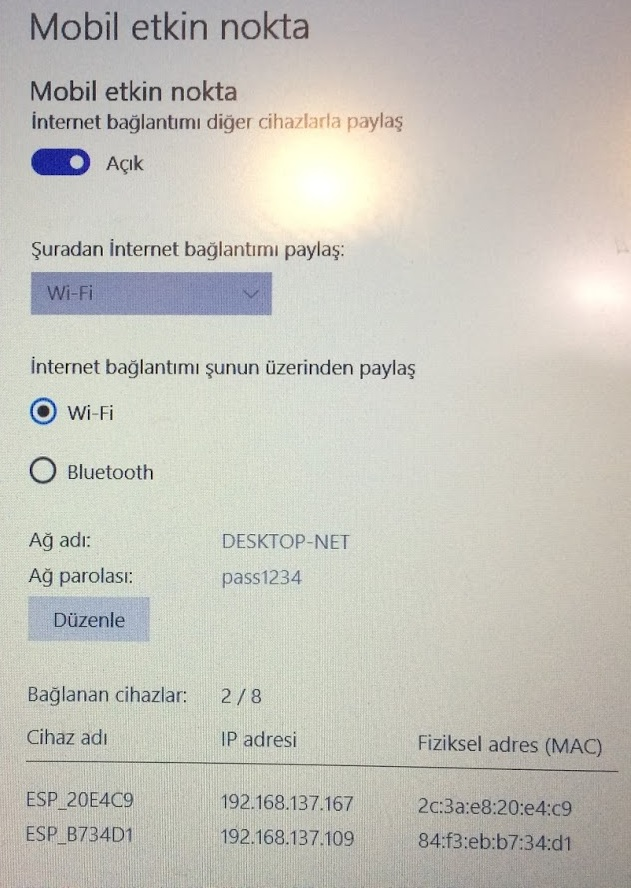
\includegraphics[width=0.4\unitlength]{images/laptop-esp-wifi}
	\caption{\label{fig:laptop-esp-wifi}Connection of ESP Modules to Laptop Hotspot.}
\end{figure}

\section{Deploying DHT11 on ESP8266}
DHT11 must be connected to the GPIO pin of the ESP module so that the temperature can be sent over Wi-Fi. This process is realized on a breadboard and explained in my GitHub repository \cite{ref-starGithub} that is dedicated for this STAR Project.
\begin{figure}[h]
	\center
	\setlength{\unitlength}{\textwidth} 
	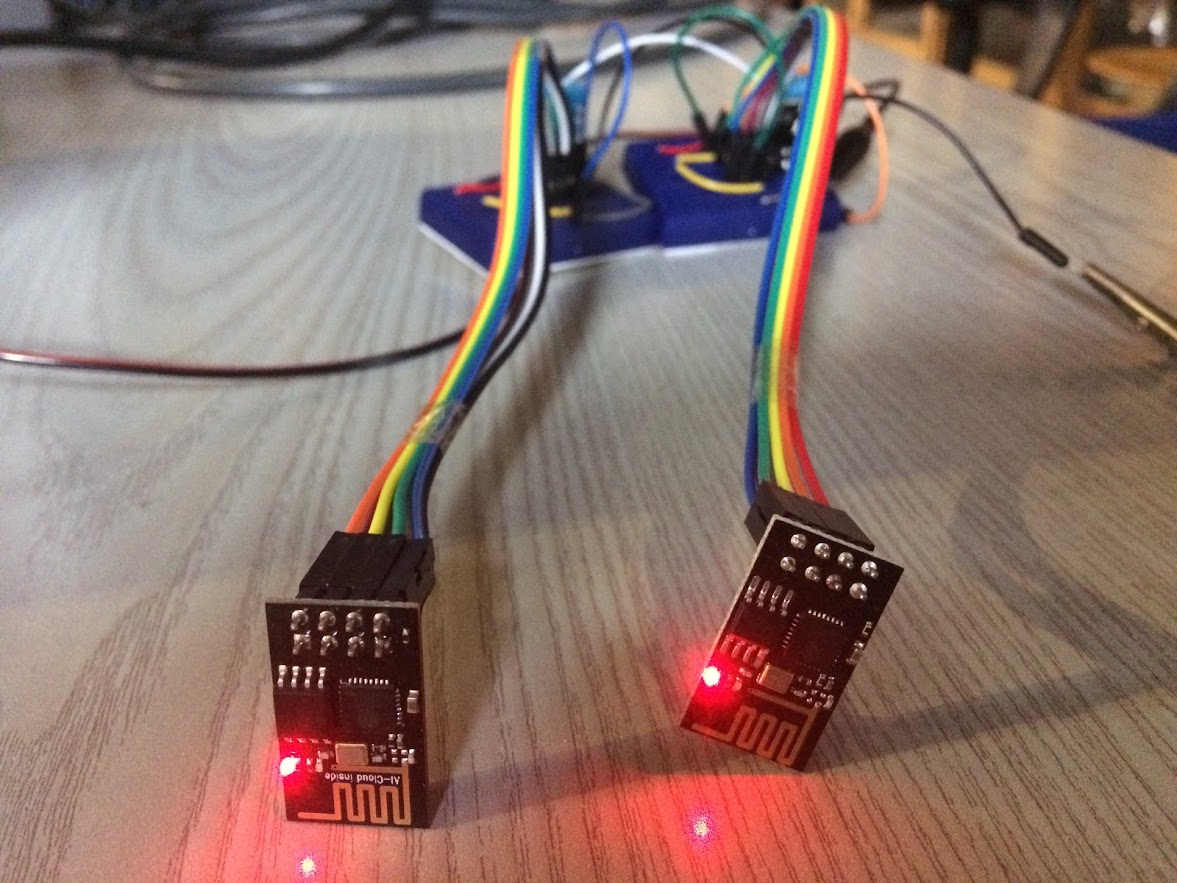
\includegraphics[width=0.4\unitlength]{images/esp-modules}
	\caption{\label{fig:esp-modules}Deployment of DHT11 and ESP8266.}
\end{figure}
\section{Test: Data Transfer Over Wi-Fi}
This test aims to test if the sensor network can send data to a broker and each other. In this test, a publicly available MQTT broker belonging to HiveMQ is used. Data transfer is successful wih a delay of 1 minutes in average. Sample screenshots are not available (I forgot to take a picture). As a last step, modules can be run using 3.7V batteries.


\section{Future Plans}
As future work, the effect of the ventilator to the temperature difference should be analyzed. Ventilator should be run according to the temperature difference measured by the sensors, however inaccuracy of the temperature sensors may cause yielding wrong conclusions. Moreover a controller will be developed according to data gathered in previous steps.

\newpage
\begin{thebibliography}{}
	\addcontentsline{toc}{section}{References}
	
	%\bibitem{ex1} "Article Title," Website Title.
	% [Online].
	%  Available: website.
	% [Accessed: 24-Sep-2017].
	
	%\bibitem{mic-ref} Agarwal, Anant. Foundations of Analog and Digital Electronic %Circuits.Department of Electrical Engineering and Computer Science, Massachusetts %Institute of Technology, 2005, p. 43
	 \bibitem{ref-dht11} [Online].
	 Available: https://www.adafruit.com/product/386.
	 [Accessed: 30-Dec-2018].
	 
	 \bibitem{ref-github-esp8266} [Online].
	 Available: https://github.com/esp8266/Arduino/issues/1032.
	 [Accessed: 30-Dec-2018].
	 
	 \bibitem{ref-mqtt} [Online].
	Available: http://mqtt.org/.
	[Accessed: 30-Dec-2018].
	 
	 \bibitem{ref-starGithub} [Online].
	Available: https://github.com/erdemtuna/METU-EE-STAR-Project.
	[Accessed: 30-Dec-2018].
	
	 \bibitem{ref-starGithub} [Online].
Available: http://www.mqtt-dashboard.com/http://www.mqtt-dashboard.com/.
[Accessed: 30-Dec-2018].


		
\end{thebibliography}

\end{document}

%----samples------
%\begin{itemize}
%\item Item
%\item Item
%\end{itemize}

%\begin{figure}[H]
%\center
%\setlength{\unitlength}{\textwidth} 
%\includegraphics[width=0.7\unitlength]{images/logo1}
%\caption{\label{fig:logo}Logo }
%\end{figure}

%\begin{figure}[H]
%	\setlength{\unitlength}{\textwidth} 
%	\centering
%	\begin{subfigure}{.5\textwidth}
%  		\centering
%  		\includegraphics[width=0.48\unitlength]{images/logo1}
%  		\caption{\label{fig:logo1}Logo1 }
%	\end{subfigure}%
%	\begin{subfigure}{.5\textwidth}
%  		\centering
%		\includegraphics[width=0.48\unitlength]{images/logo2}
%  		\caption{\label{fig:logo2}Logo2}
%	\end{subfigure}
%\caption{\label{fig:calisandegree} Small Logos   }
%\end{figure}
	
%\begin{table}[H]
%  \centering
% 
%    \begin{tabular}{c|c|c}
%       $$A$$ & $$B$$ & $$C$$ \\ \hline
%       1 & 2 & 3  \\ \hline
%       2 & 3 & 4  \\ \hline
%       3 & 4 & 5  \\ \hline
%       4 & 5 & 6  
%      
%  \end{tabular}
%  \caption{table}
%  \label{tab:table}
%\end{table}
	
%\begin{table}[H]
%  \centering
% 
%    \begin{tabular}{c|c|c}
%       \backslashbox{$A$}{$a$} & $$\specialcell{ Average deviation \\ after subtracting out the  \\ frequency error }$$ & $$C$$ \\ \hline
%       \multirow{2}{*}{1} & 2 & 3  \\ \cline{2-3}
%        & 3 & 4  \\ \hline
%       3 & \multicolumn{2}{c}{4}  \\ \hline
%       4 & 5 & 6  
%      
%  \end{tabular}
%  \caption{table}
%  \label{tab:table}
%\end{table}
%-----end of samples-----